\documentclass[tikz,border=6pt]{standalone}
\usepackage{lmodern}
\usepackage[T1]{fontenc}
\usepackage{amssymb}
\usepackage{amsmath}
\usetikzlibrary{arrows.meta,shapes.geometric,fit,backgrounds,calc,positioning,decorations.pathreplacing}
\definecolor{letterA}{HTML}{1F5FA9}
\definecolor{letterB}{HTML}{B5651D}
\definecolor{boxline}{HTML}{B9BEC4}
\definecolor{boxfill}{HTML}{F4F5F7}
\definecolor{kernel}{HTML}{3A3F45}
\definecolor{thetaT}{HTML}{2E7D46}
\definecolor{thetaF}{HTML}{C1443C}
\definecolor{xval}{HTML}{5A6470}
\definecolor{ref}{HTML}{8A9099}
\definecolor{ink}{HTML}{222629}
\tikzset{
  % ---- classes ---------------------------------------------------
  cls/.style        = {circle, draw=ink, line width=.5pt, fill=white,
                       inner sep=0pt, minimum size=13mm, align=center,
                       font=\small},
  bottom/.style     = {cls, double, double distance=1pt},
  kern/.style       = {draw=kernel, line width=1.6pt},
  % ---- SCC boxes -------------------------------------------------
  sccbox/.style     = {rounded corners=3pt, draw=boxline, fill=boxfill,
                       line width=.7pt},
  scctag/.style     = {font=\scriptsize\itshape, text=ref, align=center},
  % ---- alphabet edges --------------------------------------------
  ea/.style         = {draw=letterA, text=letterA, line width=.9pt,
                       -{Stealth[length=2mm]}},
  eb/.style         = {draw=letterB, text=letterB, line width=.9pt,
                       dashed, dash pattern=on 2.4pt off 1.6pt,
                       -{Stealth[length=2mm]}},
  eall/.style       = {draw=ink, text=ink, line width=.9pt,
                       -{Stealth[length=2mm]}},
  elab/.style       = {font=\scriptsize, inner sep=1.5pt,
                       fill=white, fill opacity=.85, text opacity=1},
  % ---- read-off decorations --------------------------------------
  thetaT/.style     = {circle, fill=thetaT, text=white, inner sep=0pt,
                       minimum size=4mm, font=\tiny\bfseries},
  thetaF/.style     = {circle, fill=thetaF, text=white, inner sep=0pt,
                       minimum size=4mm, font=\tiny\bfseries},
  xann/.style       = {font=\footnotesize, text=xval},
  result/.style     = {font=\small, text=ink},
  % ---- word ruler / verdict panels (FIG-2, FIG-3) ----------------
  cut/.style        = {draw=ref, line width=.8pt},
  jcut/.style       = {draw=ink, line width=1.1pt},
  cell/.style       = {font=\small\ttfamily, text=ink, inner sep=1pt},
  hi/.style         = {rounded corners=1pt, fill=letterA, fill opacity=.14},
  brk/.style        = {draw=ref, line width=.7pt,
                       decorate, decoration={brace, amplitude=4pt}},
  vrow/.style       = {font=\small, text=ink, anchor=west},
  vnote/.style      = {font=\scriptsize\itshape, text=ref, anchor=west},
}

\begin{document}
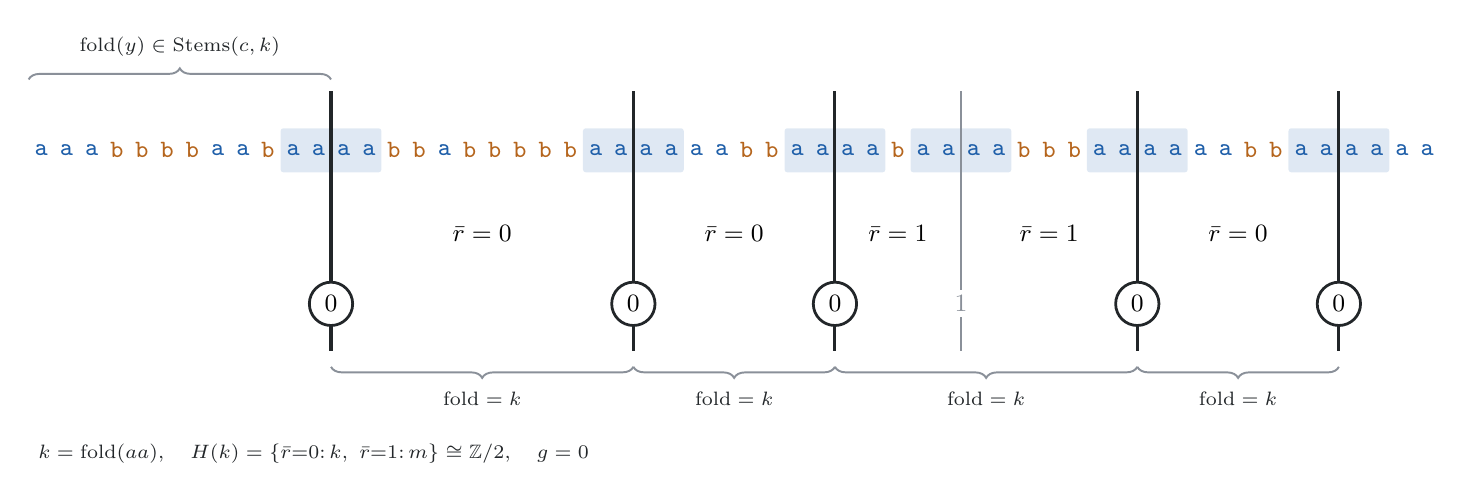
\begin{tikzpicture}
  \fill[hi] (3.20,-0.28) rectangle (4.48,0.28);
  \fill[hi] (7.04,-0.28) rectangle (8.32,0.28);
  \fill[hi] (9.60,-0.28) rectangle (10.88,0.28);
  \fill[hi] (11.20,-0.28) rectangle (12.48,0.28);
  \fill[hi] (13.44,-0.28) rectangle (14.72,0.28);
  \fill[hi] (16.00,-0.28) rectangle (17.28,0.28);
  \node[cell, text=letterA] at (0.16,0.00) {a};
  \node[cell, text=letterA] at (0.48,0.00) {a};
  \node[cell, text=letterA] at (0.80,0.00) {a};
  \node[cell, text=letterB] at (1.12,0.00) {b};
  \node[cell, text=letterB] at (1.44,0.00) {b};
  \node[cell, text=letterB] at (1.76,0.00) {b};
  \node[cell, text=letterB] at (2.08,0.00) {b};
  \node[cell, text=letterA] at (2.40,0.00) {a};
  \node[cell, text=letterA] at (2.72,0.00) {a};
  \node[cell, text=letterB] at (3.04,0.00) {b};
  \node[cell, text=letterA] at (3.36,0.00) {a};
  \node[cell, text=letterA] at (3.68,0.00) {a};
  \node[cell, text=letterA] at (4.00,0.00) {a};
  \node[cell, text=letterA] at (4.32,0.00) {a};
  \node[cell, text=letterB] at (4.64,0.00) {b};
  \node[cell, text=letterB] at (4.96,0.00) {b};
  \node[cell, text=letterA] at (5.28,0.00) {a};
  \node[cell, text=letterB] at (5.60,0.00) {b};
  \node[cell, text=letterB] at (5.92,0.00) {b};
  \node[cell, text=letterB] at (6.24,0.00) {b};
  \node[cell, text=letterB] at (6.56,0.00) {b};
  \node[cell, text=letterB] at (6.88,0.00) {b};
  \node[cell, text=letterA] at (7.20,0.00) {a};
  \node[cell, text=letterA] at (7.52,0.00) {a};
  \node[cell, text=letterA] at (7.84,0.00) {a};
  \node[cell, text=letterA] at (8.16,0.00) {a};
  \node[cell, text=letterA] at (8.48,0.00) {a};
  \node[cell, text=letterA] at (8.80,0.00) {a};
  \node[cell, text=letterB] at (9.12,0.00) {b};
  \node[cell, text=letterB] at (9.44,0.00) {b};
  \node[cell, text=letterA] at (9.76,0.00) {a};
  \node[cell, text=letterA] at (10.08,0.00) {a};
  \node[cell, text=letterA] at (10.40,0.00) {a};
  \node[cell, text=letterA] at (10.72,0.00) {a};
  \node[cell, text=letterB] at (11.04,0.00) {b};
  \node[cell, text=letterA] at (11.36,0.00) {a};
  \node[cell, text=letterA] at (11.68,0.00) {a};
  \node[cell, text=letterA] at (12.00,0.00) {a};
  \node[cell, text=letterA] at (12.32,0.00) {a};
  \node[cell, text=letterB] at (12.64,0.00) {b};
  \node[cell, text=letterB] at (12.96,0.00) {b};
  \node[cell, text=letterB] at (13.28,0.00) {b};
  \node[cell, text=letterA] at (13.60,0.00) {a};
  \node[cell, text=letterA] at (13.92,0.00) {a};
  \node[cell, text=letterA] at (14.24,0.00) {a};
  \node[cell, text=letterA] at (14.56,0.00) {a};
  \node[cell, text=letterA] at (14.88,0.00) {a};
  \node[cell, text=letterA] at (15.20,0.00) {a};
  \node[cell, text=letterB] at (15.52,0.00) {b};
  \node[cell, text=letterB] at (15.84,0.00) {b};
  \node[cell, text=letterA] at (16.16,0.00) {a};
  \node[cell, text=letterA] at (16.48,0.00) {a};
  \node[cell, text=letterA] at (16.80,0.00) {a};
  \node[cell, text=letterA] at (17.12,0.00) {a};
  \node[cell, text=letterA] at (17.44,0.00) {a};
  \node[cell, text=letterA] at (17.76,0.00) {a};
  \draw[jcut] (3.84,0.75) -- (3.84,-2.55);
  \draw[jcut] (7.68,0.75) -- (7.68,-2.55);
  \draw[jcut] (10.24,0.75) -- (10.24,-2.55);
  \draw[cut] (11.84,0.75) -- (11.84,-2.55);
  \draw[jcut] (14.08,0.75) -- (14.08,-2.55);
  \draw[jcut] (16.64,0.75) -- (16.64,-2.55);
  \node[font=\small] at (5.76,-1.05) {$\bar r=0$};
  \node[font=\small] at (8.96,-1.05) {$\bar r=0$};
  \node[font=\small] at (11.04,-1.05) {$\bar r=1$};
  \node[font=\small] at (12.96,-1.05) {$\bar r=1$};
  \node[font=\small] at (15.36,-1.05) {$\bar r=0$};
  \node[circle,draw=ink,line width=1pt,inner sep=1pt,minimum size=5.5mm,font=\small,fill=white] at (3.84,-1.95) {$0$};
  \node[circle,draw=ink,line width=1pt,inner sep=1pt,minimum size=5.5mm,font=\small,fill=white] at (7.68,-1.95) {$0$};
  \node[circle,draw=ink,line width=1pt,inner sep=1pt,minimum size=5.5mm,font=\small,fill=white] at (10.24,-1.95) {$0$};
  \node[font=\small,text=ref,fill=white,inner sep=2pt] at (11.84,-1.95) {$1$};
  \node[circle,draw=ink,line width=1pt,inner sep=1pt,minimum size=5.5mm,font=\small,fill=white] at (14.08,-1.95) {$0$};
  \node[circle,draw=ink,line width=1pt,inner sep=1pt,minimum size=5.5mm,font=\small,fill=white] at (16.64,-1.95) {$0$};
  \draw[brk] (7.68,-2.75) -- (3.84,-2.75);
  \node[font=\scriptsize,text=ink] at (5.76,-3.15) {$\mathrm{fold}=k$};
  \draw[brk] (10.24,-2.75) -- (7.68,-2.75);
  \node[font=\scriptsize,text=ink] at (8.96,-3.15) {$\mathrm{fold}=k$};
  \draw[brk] (14.08,-2.75) -- (10.24,-2.75);
  \node[font=\scriptsize,text=ink] at (12.16,-3.15) {$\mathrm{fold}=k$};
  \draw[brk] (16.64,-2.75) -- (14.08,-2.75);
  \node[font=\scriptsize,text=ink] at (15.36,-3.15) {$\mathrm{fold}=k$};
  \draw[brk] (0.00,0.90) -- (3.84,0.90);
  \node[font=\scriptsize,text=ink,anchor=south] at (1.92,1.07) {fold$(y)\in\mathrm{Stems}(c,k)$};
  \node[font=\scriptsize,text=ink,anchor=west] at (0.00,-3.85) {$k=\mathrm{fold}(aa),\quad H(k)=\{\bar r{=}0{:}\,k,\ \bar r{=}1{:}\,m\}\cong\mathbb{Z}/2,\quad g=0$};
\end{tikzpicture}
\end{document}
